\documentclass[abstracton,12pt]{scrreprt}

\usepackage[utf8]{inputenc}
\usepackage[T1]{fontenc}
\usepackage{fancyhdr}
\usepackage{graphicx}
\usepackage{tikz}
\usepackage{times}
\usepackage{listings}
\usepackage{amssymb}
\usepackage{amsfonts}
\usepackage{amsmath}

% --------- 

\titlehead{Department of Informatics, University of Zürich}
\subject{\vspace*{2cm}MSc Thesis}
\title{Replace by Title of your Thesis}
\author{
  Put Your Name\\[-5pt]
  \scriptsize Matrikelnummer: xx-xxx-xxx\\[-5pt]
  \scriptsize Email: \texttt{xxx@yyy}
}
\date{\vspace*{2cm}January 11, 2010}
\publishers{
  \small supervised by Prof.\ Dr.\ x.\ yyy and y.\ zzz \\[5cm]
  \begin{tikzpicture}[overlay]
    \node at (-3,-3) {\includegraphics[height=1.5cm]{IFIlogo}};
    \node at (7,-3) {\includegraphics[height=1.5cm]{dbtgBW}};
  \end{tikzpicture}
}

\dedication{dedicated to xxx}

% --------- 

\newtheorem{definition}{Definition}
\newtheorem{example}{Example}
\newtheorem{theorem}{Theorem}
\newtheorem{lemma}{Lemma}

\newenvironment{proof}
  {\noindent{\bf Proof:\rm}}{\hfill$\Box$\vspace{\medskipamount}}

\def\bbbr{{\rm I\!R}}
\def\bbbm{{\rm I\!M}}
\def\bbbn{{\rm I\!N}}
\def\bbbz{{\rm I\!Z}}

% --------- 

\begin{document}

\maketitle

\chapter*{Acknowledgements}

\begin{abstract}
  ...
\end{abstract}

\chapter*{Zusammenfassung}

\tableofcontents
\listoffigures
\listoftables

\chapter{Introduction}

\section{Fixed-Period Problems: The Sublinear Case}

With this chapter, the preliminaries are over, and we begin the search
for periodic solutions to Hamiltonian systems. All this will be done
in the convex case; that is, we shall study the boundary-value problem
\begin{eqnarray*}
  \dot{x}&=&JH' (t,x)\\
  x(0) &=& x(T)
\end{eqnarray*}
with $H(t,\cdot)$ a convex function of $x$, going to $+\infty$ when
$\left\|x\right\| \to \infty$.

\begin{example} [{\rm(External forcing)}]
Consider the system:
\begin{equation}
  \dot{x} = JH' (x) + f(t)
\end{equation}
where the Hamiltonian $H$ is $\left(0,b_{\infty}\right)$-subquadratic,
and the forcing term is a distribution on the circle.
\end{example}

\subsection{Autonomous Systems}

We assume a \emph{time domain}, $\mathcal{A}$, as a set of time
instants equipped with a total order $\leq$ and isomorph to integers.
Time granularities are partitionings of subsets of $\mathcal{A}$ into
non-empty intervals of time instants, termed \emph{granules}.
Examples of time granularities are minutes ($\mathit{min}$), hours
($\mathit{hou}$), days ($\mathit{day}$), weeks ($\mathit{wee}$),
months ($\mathit{mth}$), and years ($\mathit{yea}$).  The granularity
$\mathit{day}$, for instance, divides the time domain into granules of
1440 minutes.  We assume a \emph{bottom granularity}, $G_\bot$, such
that each granule of $G_\bot$ contains exactly one time instant.  In
our running example minutes represent the bottom granularity, and we
use the ISO~8601:2004 notation to denote time instants, e.g.,
\mbox{2007-02-12 07:15}.  The granules of each granularity $G$ are
ordered according to the time domain order and indexed with a subset
of integers, $\mathcal{L}_G$, such that the indexing function
$\mathcal{M}_G : \mathcal{L}_G \to G$ is an isomorphism that preserves
the total order $\leq$. For each granularity we assume that the
granule with index~0 contains the time instant 2000-01-01-00:00.
Figure~\ref{fig:ch0-gran-labels} illustrates some correspondences of
indexes between different granularities, e.g.,
$\mathcal{M}_\mathit{day}(2599)$ = [2007-02-12 00:00, 2007-02-12
23:59].

For the conversion between different granularities, we adopt the
\emph{bigger-part-inside semantics}~\cite{Ohlbach06,ical98}.  The
conversion from a coarser granularity $H$ to a finer granularity $G$
is defined as
\begin{align*}
  \downharpoonright^{H}_{G}(i) = \{ j \mid
  & |\mathcal{M}_{G}(j) \cap
  \mathcal{M}_{H}(i)| > |\mathcal{M}_{G}(j) \setminus
  \mathcal{M}_{H}(i)| \lor {}
  \\
  & (|\mathcal{M}_{G}(j) \cap \mathcal{M}_{H}(i)| =
  |\mathcal{M}_{G}(j) \setminus \mathcal{M}_{H}(i)| \land
  \max(\mathcal{M}_{G}(j)) \in \mathcal{M}_{H}(i) )\}
\end{align*}
$\downharpoonright^{H}_{G}(i)$ returns the indexes of those granules
in $G$ that are covered by granule $i$ in $H$ for more than a half or,
if exactly half of a granule in $G$ is covered, the second half.

\section{Time Slices and Multislices}

A (time) \emph{slice}~\cite{Niezette92} is a finite list of pairs,
$\lambda = (G_1X_1,\ldots,G_dX_d)$, where $G_l$ are granularities and
$X_l$ are \emph{selectors} that are defined as sets of integers.  Each
selector $X_{l+1}$ specifies a set of granules in $G_{l+1}$ with a
relative positioning with respect to granularity $G_l$.  The sequence
of granularities $(G_1,\ldots,G_d)$ is the \emph{hierarchy} of the
slice.  

Consider the slice $(\mathit{yea}\{7\}, \mathit{wee}\{\text{0-25}\},
\mathit{day}\{\text{0-4}\}, \mathit{hou}\{7\},
\mathit{min}\{\text{0,25,55}\})$.  The hierarchy is $(\mathit{wee},
\mathit{day}, \mathit{hou}, \mathit{min})$.  The first selector
$\{7\}$ selects the year 2007, the selector \{0-25\} selects the first
26 weeks of this year, the selector \{0-4\} selects the days from
Monday to Friday from each of these weeks, etc.

The semantics of a slice $\lambda$ = $(G_1X_1$, \ldots, $G_dX_d)$ is
defined through the following mapping $\mathcal{I}$ to a subset of the
time domain:

\begin{equation*}
  \mathcal{I} (\lambda) =
  \begin{cases}
    \bigcup_{k \in X_1} \mathcal{M}_{G_1}(k) & d=1 \\[1ex]
    \mathcal{I} \left( (G_2\bigcup_{k \in X_1}(
      \downharpoonright^{G_1}_{G_2}(k)/^+X_2), \ldots, G_dX_d)
    \right) & d>1
  \end{cases}
\end{equation*}

Here, $\downharpoonright^{G_1}_{G_2}$ is a bigger-part-inside
conversion from a granularity $G_1$ to a granularity $G_2$, and
$\downharpoonright^{G_1}_{G_2}(k)/^+X_2$ is defined as
$\downharpoonright^{G_1}_{G_2}(k) \cap \{
\min(\downharpoonright^{G_1}_{G_2}(k)) + i \mid i \in X_2 \}$.

\begin{figure}[htbp]\centering
  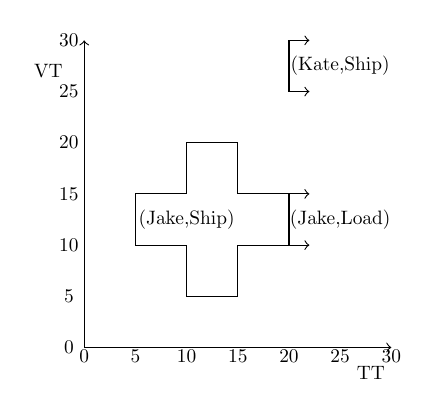
\begin{tikzpicture}[scale=0.13]
    \tikzstyle{every node}=[scale=0.7]
    \draw[->] (0,0) -- (30,0);
    \foreach \t in {0,5,10,15,20,25,30} \node at (\t,-0.9) {\t};
    \draw (28,-2.5) node {TT};
    \draw[->] (0,0) -- (0,30);
    \foreach \t in {0,5,10,15,20,25,30} \node at (-1.5,\t) {\t};
    \draw (-3.5,27) node {VT};
    \draw[<->] (22,10) -- (15,10) -- (15,5) -- (10,5) -- (10,10)
      -- (5,10) -- (5,15) -- (10,15) -- (10,20) -- (15,20) -- (15,15)
      -- (22,15);
    \draw (20,10) -- (20,15);
    \draw (10,12.5) node {(Jake,Ship)};
    \draw (25,12.5) node {(Jake,Load)};
    \draw[<->] (22,25) -- (20,25) -- (20,30) -- (22,30);
    \draw (25,27.5) node {(Kate,Ship)};
  \end{tikzpicture}
  \caption{Relationships between $P$, $M$, and $M_\mathrm{min}$}
  \label{fig:ch2-singular-minimal-mapping}
\end{figure}

\chapter{The Final One}

\begin{lemma}
Assume that $H$ is $C^{2}$ on $\bbbr^{2n} \setminus \{ 0\}$ and
that $H'' (x)$ is non-de\-gen\-er\-ate for any $x\ne 0$. Then any local
minimizer $\widetilde{qx}$ of $\psi$ has minimal period $T$.
\end{lemma}

\begin{proof}
We know that $\widetilde{x}$, or
$\widetilde{x} + \xi$ for some constant $\xi
\in \bbbr^{2n}$, is a $T$-periodic solution of the Hamiltonian system:
\begin{equation}
  \dot{x} = JH' (x)\ .
\end{equation}

There is no loss of generality in taking $\xi = 0$. So
$\psi (x) \ge \psi (\widetilde{x} )$
for all $\widetilde{x}$ in some neighbourhood of $x$ in
$W^{1,2} \left(\bbbr / T\bbbz ; \bbbr^{2n}\right)$.

But this index is precisely the index
$i_{T} (\widetilde{x} )$ of the $T$-periodic
solution $\widetilde{x}$ over the interval
$(0,T)$, as defined in Sect.~2.6. So
\begin{equation}
  i_{T} (\widetilde{x} ) = 0\ .
  \label{eq:five}
\end{equation}

Now if $\widetilde{x}$ has a lower period, $T/k$ say,
we would have, by Corollary 31:
\begin{equation}
  i_{T} (\widetilde{x} ) =
  i_{kT/k}(\widetilde{x} ) \ge
  ki_{T/k} (\widetilde{x} ) + k-1 \ge k-1 \ge 1\ .
\end{equation}

This would contradict (~\ref{eq:five}), and thus cannot happen.
\end{proof}

\begin{figure}[htbp]\centering
  \includegraphics{dbtgBW}
  \caption{DBTGlogo}
  \label{fig:dbtglogo}
\end{figure}

A reference to a Figure~\ref{fig:dbtglogo}.

\bibliographystyle{alpha}
\bibliography{}

\end{document}
